\documentclass[aspectratio=169]{beamer}
\usetheme{Madrid}
\usecolortheme{beaver}
\usepackage[utf8]{inputenc}
\usepackage[T1]{fontenc}
\usepackage{tikz}
\usepackage{amssymb}
\usepackage{graphicx}
\setbeamertemplate{navigation symbols}{}
\setbeamercolor{title}{fg=white,bg=cyan!60!black}
\setbeamercolor{frametitle}{fg=white,bg=cyan!50!black}
\setbeamercolor{block title}{bg=cyan!15,fg=black}
\setbeamercolor{block body}{bg=cyan!5,fg=black}

\title{G1 — Sprite Start}
\subtitle{BOSS: Sprite Follows You}
\author{ByteForge --- Grade 7 --- Game Maker}
\date{}

\begin{document}

\begin{frame}
    \titlepage
\end{frame}

\begin{frame}{BOSS — coordinates that update every frame}
    \Large
    "On every frame" re-runs its contents dozens of times a second — clear, then redraw, every frame, is the engine behind every animated game.

    \begin{center}
    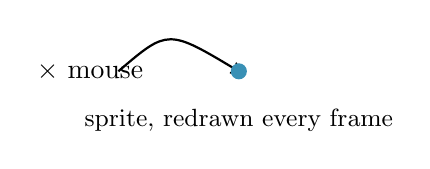
\begin{tikzpicture}[scale=0.9]

        \node at (0.9,-1) {$\times$ mouse};
        \draw[->, thick] (1.3,-1) .. controls (2,-0.4) .. (3,-1);
        \filldraw[cyan!70!black] (3,-1) circle (3pt);
        \node[below] at (3,-1.4) {\small sprite, redrawn every frame};
    \end{tikzpicture}
    \end{center}
\end{frame}

\begin{frame}{Your Turn}
    \Large
    Open the student map, find \textbf{G1 — Sprite Start}, and complete
    the \textbf{BOSS} challenge --- everything you just saw, they now do themselves.
\end{frame}

\end{document}
